\documentclass{beamer}
\usepackage{tikz, xcolor}
\usetikzlibrary{arrows.meta}
\usetheme{default}
\setbeamertemplate{headline}{%
\begin{beamercolorbox}[wd=\paperwidth,ht=3ex,dp=1ex,center]{section in head/foot}%
\usebeamercolor[fg]{section in head/foot}%
Operations Research
\end{beamercolorbox}%
}

\setbeamercolor{section in head/foot}{bg=blue!50, fg=white}
\begin{document}

\begin{frame}{Graph}
    \begin{center}
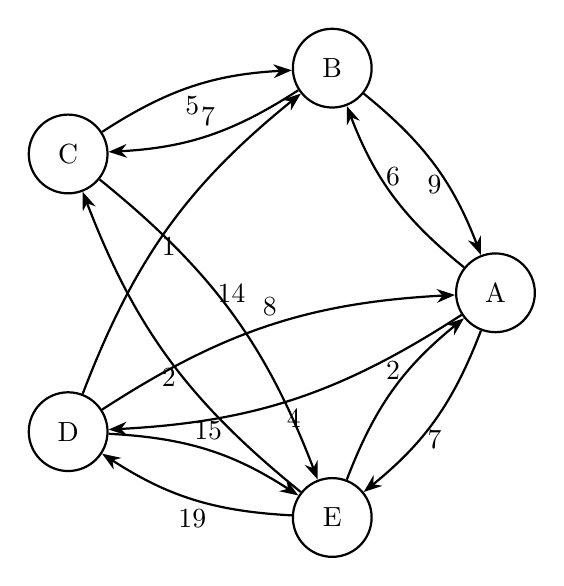
\begin{tikzpicture}[->, >=Stealth, thick, main/.style={circle, draw, minimum size=1cm}]

    \node[main] (A) at (0.00:3cm) {A};
    \node[main] (B) at (72.00:3cm) {B};
    \node[main] (C) at (144.00:3cm) {C};
    \node[main] (D) at (216.00:3cm) {D};
    \node[main] (E) at (288.00:3cm) {E};
\path
        (A) edge[bend left=15] node[above, fill=none] {6} (B)
        (A) edge[bend left=15] node[below, fill=none] {4} (D)
        (A) edge[bend left=15] node[below, fill=none] {7} (E)
        (B) edge[bend left=15] node[below, fill=none] {9} (A)
        (B) edge[bend left=15] node[above, fill=none] {7} (C)
        (C) edge[bend left=15] node[below, fill=none] {5} (B)
        (C) edge[bend left=15] node[above, fill=none] {14} (E)
        (D) edge[bend left=15] node[above, fill=none] {8} (A)
        (D) edge[bend left=15] node[below, fill=none] {1} (B)
        (D) edge[bend left=15] node[above, fill=none] {15} (E)
        (E) edge[bend left=15] node[above, fill=none] {2} (A)
        (E) edge[bend left=15] node[below, fill=none] {2} (C)
        (E) edge[bend left=15] node[below, fill=none] {19} (D)
;
\end{tikzpicture}
\end{center}
\end{frame}

\begin{frame}{Table D(0)}
    \begin{center}
        \begin{tabular}{c|ccccc}
         & v1 & v2 & v3 & v4 & v5 \\
\hline
v1 & 0 & 6 & $\infty$ & 4 & 7 \\
v2 & 9 & 0 & 7 & $\infty$ & $\infty$ \\
v3 & $\infty$ & 5 & 0 & $\infty$ & 14 \\
v4 & 8 & 1 & $\infty$ & 0 & 15 \\
v5 & 2 & $\infty$ & 2 & 19 & 0 \\
        \end{tabular}
    \end{center}
\end{frame}

\begin{frame}{Table D(1)}
    \begin{center}
        \begin{tabular}{c|ccccc}
         & v1 & v2 & v3 & v4 & v5 \\
\hline
v1 & 0 & 6 & $\infty$ & 4 & 7 \\
v2 & 9 & 0 & 7 & \textcolor{blue}{13} & \textcolor{blue}{16} \\
v3 & $\infty$ & 5 & 0 & $\infty$ & 14 \\
v4 & 8 & 1 & $\infty$ & 0 & 15 \\
v5 & 2 & \textcolor{blue}{8} & 2 & \textcolor{blue}{6} & 0 \\
        \end{tabular}
    \end{center}
\end{frame}

\begin{frame}{Table P}
    \begin{center}
        \begin{tabular}{c|ccccc}
         & v1 & v2 & v3 & v4 & v5 \\
\hline
v1 & 0 & 0 & 0 & 0 & 0 \\
v2 & 0 & 0 & 0 & \textcolor{blue}{1} & \textcolor{blue}{1} \\
v3 & 0 & 0 & 0 & 0 & 0 \\
v4 & 0 & 0 & 0 & 0 & 0 \\
v5 & 0 & \textcolor{blue}{1} & 0 & \textcolor{blue}{1} & 0 \\
        \end{tabular}
    \end{center}
\end{frame}

\begin{frame}{Table D(2)}
    \begin{center}
        \begin{tabular}{c|ccccc}
         & v1 & v2 & v3 & v4 & v5 \\
\hline
v1 & 0 & 6 & \textcolor{blue}{13} & 4 & 7 \\
v2 & 9 & 0 & 7 & 13 & 16 \\
v3 & \textcolor{blue}{14} & 5 & 0 & \textcolor{blue}{18} & 14 \\
v4 & 8 & 1 & \textcolor{blue}{8} & 0 & 15 \\
v5 & 2 & 8 & 2 & 6 & 0 \\
        \end{tabular}
    \end{center}
\end{frame}

\begin{frame}{Table P}
    \begin{center}
        \begin{tabular}{c|ccccc}
         & v1 & v2 & v3 & v4 & v5 \\
\hline
v1 & 0 & 0 & \textcolor{blue}{2} & 0 & 0 \\
v2 & 0 & 0 & 0 & 1 & 1 \\
v3 & \textcolor{blue}{2} & 0 & 0 & \textcolor{blue}{2} & 0 \\
v4 & 0 & 0 & \textcolor{blue}{2} & 0 & 0 \\
v5 & 0 & 1 & 0 & 1 & 0 \\
        \end{tabular}
    \end{center}
\end{frame}

\begin{frame}{Table D(3)}
    \begin{center}
        \begin{tabular}{c|ccccc}
         & v1 & v2 & v3 & v4 & v5 \\
\hline
v1 & 0 & 6 & 13 & 4 & 7 \\
v2 & 9 & 0 & 7 & 13 & 16 \\
v3 & 14 & 5 & 0 & 18 & 14 \\
v4 & 8 & 1 & 8 & 0 & 15 \\
v5 & 2 & \textcolor{blue}{7} & 2 & 6 & 0 \\
        \end{tabular}
    \end{center}
\end{frame}

\begin{frame}{Table P}
    \begin{center}
        \begin{tabular}{c|ccccc}
         & v1 & v2 & v3 & v4 & v5 \\
\hline
v1 & 0 & 0 & 2 & 0 & 0 \\
v2 & 0 & 0 & 0 & 1 & 1 \\
v3 & 2 & 0 & 0 & 2 & 0 \\
v4 & 0 & 0 & 2 & 0 & 0 \\
v5 & 0 & \textcolor{blue}{3} & 0 & 1 & 0 \\
        \end{tabular}
    \end{center}
\end{frame}

\begin{frame}{Table D(4)}
    \begin{center}
        \begin{tabular}{c|ccccc}
         & v1 & v2 & v3 & v4 & v5 \\
\hline
v1 & 0 & \textcolor{blue}{5} & \textcolor{blue}{12} & 4 & 7 \\
v2 & 9 & 0 & 7 & 13 & 16 \\
v3 & 14 & 5 & 0 & 18 & 14 \\
v4 & 8 & 1 & 8 & 0 & 15 \\
v5 & 2 & 7 & 2 & 6 & 0 \\
        \end{tabular}
    \end{center}
\end{frame}

\begin{frame}{Table P}
    \begin{center}
        \begin{tabular}{c|ccccc}
         & v1 & v2 & v3 & v4 & v5 \\
\hline
v1 & 0 & \textcolor{blue}{4} & \textcolor{blue}{4} & 0 & 0 \\
v2 & 0 & 0 & 0 & 1 & 1 \\
v3 & 2 & 0 & 0 & 2 & 0 \\
v4 & 0 & 0 & 2 & 0 & 0 \\
v5 & 0 & 3 & 0 & 1 & 0 \\
        \end{tabular}
    \end{center}
\end{frame}

\begin{frame}{Table D(5)}
    \begin{center}
        \begin{tabular}{c|ccccc}
         & v1 & v2 & v3 & v4 & v5 \\
\hline
v1 & 0 & 5 & \textcolor{blue}{9} & 4 & 7 \\
v2 & 9 & 0 & 7 & 13 & 16 \\
v3 & 14 & 5 & 0 & 18 & 14 \\
v4 & 8 & 1 & 8 & 0 & 15 \\
v5 & 2 & 7 & 2 & 6 & 0 \\
        \end{tabular}
    \end{center}
\end{frame}

\begin{frame}{Table P}
    \begin{center}
        \begin{tabular}{c|ccccc}
         & v1 & v2 & v3 & v4 & v5 \\
\hline
v1 & 0 & 4 & \textcolor{blue}{5} & 0 & 0 \\
v2 & 0 & 0 & 0 & 1 & 1 \\
v3 & 2 & 0 & 0 & 2 & 0 \\
v4 & 0 & 0 & 2 & 0 & 0 \\
v5 & 0 & 3 & 0 & 1 & 0 \\
        \end{tabular}
    \end{center}
\end{frame}

\begin{frame}{Shortest Paths from v1}
\begin{itemize}
    \item to v2 (5): v1 $\rightarrow$ v4 $\rightarrow$ v2
\item to v3 (9): v1 $\rightarrow$ v5 $\rightarrow$ v3
\item to v4 (4): v1 $\rightarrow$ v4
\item to v5 (7): v1 $\rightarrow$ v5
\end{itemize}
\end{frame}

\begin{frame}{Shortest Paths from v2}
\begin{itemize}
    \item to v1 (9): v2 $\rightarrow$ v1
\item to v3 (7): v2 $\rightarrow$ v3
\item to v4 (13): v2 $\rightarrow$ v1 $\rightarrow$ v4
\item to v5 (16): v2 $\rightarrow$ v1 $\rightarrow$ v5
\end{itemize}
\end{frame}

\begin{frame}{Shortest Paths from v3}
\begin{itemize}
    \item to v1 (14): v3 $\rightarrow$ v2 $\rightarrow$ v1
\item to v2 (5): v3 $\rightarrow$ v2
\item to v4 (18): v3 $\rightarrow$ v2 $\rightarrow$ v1 $\rightarrow$ v4
\item to v5 (14): v3 $\rightarrow$ v5
\end{itemize}
\end{frame}

\begin{frame}{Shortest Paths from v4}
\begin{itemize}
    \item to v1 (8): v4 $\rightarrow$ v1
\item to v2 (1): v4 $\rightarrow$ v2
\item to v3 (8): v4 $\rightarrow$ v2 $\rightarrow$ v3
\item to v5 (15): v4 $\rightarrow$ v5
\end{itemize}
\end{frame}

\begin{frame}{Shortest Paths from v5}
\begin{itemize}
    \item to v1 (2): v5 $\rightarrow$ v1
\item to v2 (7): v5 $\rightarrow$ v3 $\rightarrow$ v2
\item to v3 (2): v5 $\rightarrow$ v3
\item to v4 (6): v5 $\rightarrow$ v1 $\rightarrow$ v4
\end{itemize}
\end{frame}

\end{document}